\documentclass[a4paper]{article}

\usepackage[utf8]{inputenc}
\usepackage{erk}
\usepackage{times}
\usepackage{graphicx}
\usepackage[top=22.5mm, bottom=22.5mm, left=22.5mm, right=22.5mm]{geometry}

\usepackage[slovene,english]{babel}
\usepackage{hyperref}
\usepackage{url}

\let\oldfootnotesize\footnotesize
\renewcommand*{\footnotesize}{\oldfootnotesize\scriptsize}

\begin{document}
\title{Scenarij za igro Arrrr! pri predmetu Računalniška grafika in tehnologija iger}

\author{Jernej Ko\v zelj$^{1}$, Metod Ribi\v c$^{1}$, Barbara Nagli\v c$^{2}$, Rok Kompare$^{2}$}

\affiliation{	$^{1}$Univerza v Ljubljani, Fakulteta za računalništvo in informatiko \\ 
				$^{2}$Univerza v Ljubljani, Naravoslovnotehni\v ska fakulteta }



\maketitle

\selectlanguage{slovene}

\begin{abstract}{Kratek opis igre}
Uporabnik vodi gusarsko ladjo skozi o\v zino, hkrati pa se mora izogibati razbitinam. Na poti lahko pobira nagrade v obliki zakladov, ter tako nabira to\v cke. Cilj igre je, da uporabnik pripelje ladjo nepo\v skodovano do cilja, ter na poti pobere \v cimve\v c zakladov.
\end{abstract}


\begin{figure}[!htb]
    \begin{center}
        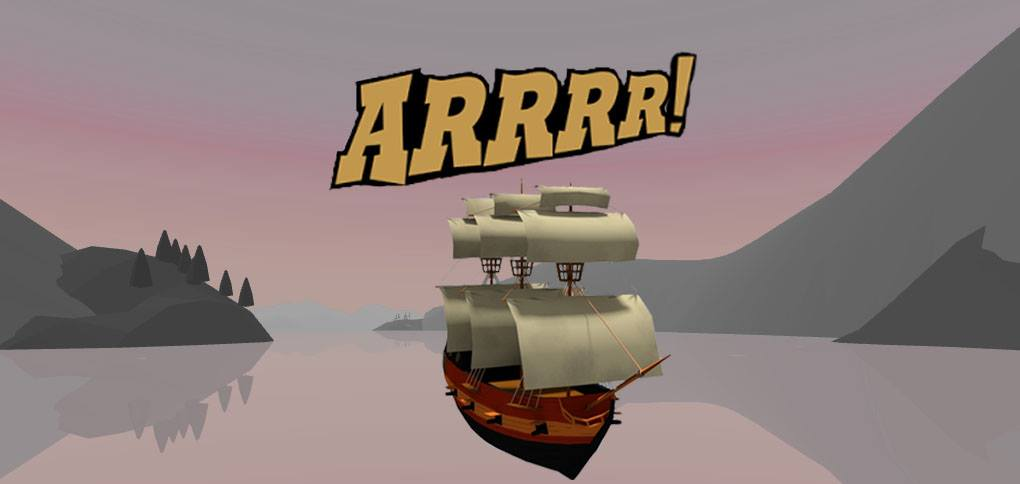
\includegraphics[width=\columnwidth]{arrr.jpg}
        \caption{Naslovna slika} \label{fig:slika}
    \end{center}
\end{figure}




\section{Pregled igre}
Igre je akcijska \textbf{\textit{(action-adventure)}}, kjer uporabnik vodi ladjo skozi mno\v zico ovir, pri \v cemer pa se te\v zavnost igre sproti pove\v cuje tako, da se ladja giblje vedno hitreje. Igra je namenjena vsem starostnim skupinam, saj je enostavna za igranje, prav tako pa spodbuja lastno \v zeljo uporabnika po \v cim bolj\v sem rezultatu.

\subsection{Opis sveta}
Igralec je postavljen v ravninski navidezen gusarski svet, ki predstavlja o\v zino po kateri mora voditi ladjo do cilja. Svet je sestavljen iz vode, gora ter objektov, ki jih mora uporabnik pobirati ali pa se jim izogibati. Svet temelji na principu \textbf{\textit{"low poly"}}, torej da se obliko dose\v ze s \v cim manj poligoni, temu primerne so tudi barve.

\subsubsection{Pregled}
Uporabnik ob zagonu igre vidi za\v cetno pozicijo ladje, ob prvem pritisku tipke levo ali desno pa spro\v zi za\v cetek igre. Na tem mestu je tudi ikona za nastavitve, kjer si uporabnik lahko nastavi poljubne nastavitve. Sama igra poteka v svetu, ki je opisan v prej\v snjem odstavku. 

\subsubsection{Ozadje}
Okolico predstavljajo gore, te pa sestavljajo o\v zino, s katero uporabnik ne more interaktirati, razen, \v ce se preve\v c pribli\v za kopnemu, kar pomeni, da uni\v ci ladjo, ter s tem svojo popotovanje do cilja.

\subsubsection{Ključne lokacije}
Glavna klju\v cna lokacija v igri za uporabnika je cilj, do katerega mora pripeljati nepo\v skodovano ladjo. Na poti pa sta klju\v cni dve lokaciji in sicer razbitine, ki se jim mora uporabnik izogibati, ter zakladi, ki prinesejo uporabniku to\v cke.

\subsubsection{Velikost}
Velikost igre je omejena na o\v zino, ki je prej definirana, ter temelji na fjordu oziroma na reliefu iz realnega sveta.

\subsubsection{Objekti}
Igra vsebuje gusarsko ladjo, razli\v cne razbitine ter zaklade. Vsi objekti so bili izdelani izklju\v cno za igro \textbf{\textit{Arrrr!}}.

\subsubsection{\v Cas}
\v Cas v igri ni definiran, saj uporabnik ni vezan na \v cas, va\v zno je le, da pride do cilja. S \v casom se pove\v cuje zahtevnost igre, uporabnik pa to vidi tako, da se ladja premika vedno hitreje.

\subsection{Igralni pogon in uporabljene tehnologije}
Za izdelavo igre je uporabljen WebGL\footnote{\url{https://get.webgl.org/}} ter knji\v znica THREE.js\footnote{\url{https://http://threejs.org/}} za interakcijo med objekti pa je uporabljena knji\v znica Physijs\footnote{\url{http://chandlerprall.github.io/Physijs/}}.

\subsection{Pogled}
V igri je uporabljena tretjeosebna kamera, uporabnik nima vpliva na velikost okolice, ki jo vidi, saj je vedno prikazan kos oklice, ki ga je zajela kamera, kamera pa se giblje po prej definirani navidezni poti.


\small
\bibliographystyle{plain}
\bibliography{references}


\end{document}
